\documentclass[class=book, crop=false]{standalone}
\usepackage[subpreambles=true]{standalone}

\usepackage{../../style}

\graphicspath{{./assets/images/}}%

\begin{document}
\chapter{L'architettura MIPS}
\section{Gestione delle procedure}
L'utilità dei calcolatori sarebbe molto limitata se questi non avessero la possibilità di svolgere delle procedure, che possono essere immaginate a tutti gli effetti come delle funzioni che dato un certo input eseguono un determinato task a cui sono dedicate.\\
L'aspetto fondamentale che si deve curare per dare la possibilità ai calcolatori di svolgere procedure è la definizione di un protocollo di chiamata delle procedure che deve stabilire con precisione questi aspetti:
\begin{itemize}[noitemsep]
	\item Come caricare i parametri di input della procedura in locazioni note
	\item Come trasferire il controllo alla procedura, che deve:
		\begin{itemize}[nolistsep, noitemsep]
			\item Acquisire le risorse necessarie
			\item Eseguire il task affidatole
			\item Caricare gli output in locazioni note
			\item Restituire il controllo al chiamante
		\end{itemize}
	\item Come salvare il valore di ritorno della procedura e "fare pulizia" del tutto
\end{itemize}
I protocolli per la gestione delle procedure sono diversi in base all'architettura che si utilizza ed alle convenzioni di chiamata del compilatore, noi per ora studiamo il caso del MIPS.

\section{Protocollo di chiamata MIPS}
L'idea fondante del protocollo implementato da MIPS è di utilizzare ogniqualvolta possibile i registri, dato che essi sono il meccanismo più veloce a disposizione per la gestione dei parametri delle procedure. Ecco una tabella riassuntiva delle convenzioni sui registri definite nel MIPS:

%\begin{table}[H]
%	\centering
%	\caption{didascalia}
%	\subimport{assets/tables/}{convenzioni-registri-MIPS.tex}
%\end{table}

Oltre ai registri il MIPS mette a disposizione dell'utente l'istruzione \emph{jump and link (jal)} che effettua il salto ???(all'esecuzione di una data funzione)??? e contemporaneamente memorizza in \emph{\$ra} l'indirizzo di ritorno ???(una volta terminata la funzione)???. Questo significa che quano si chiama la \emph{jal} si salva automaticamente in \emph{\$ra} il PC incrementato di 4 (l'iztruzione successiva).\\
Alla fine della procedura sarà così sufficiente compiere il salto \mintinline{asm}{js \$ra} per riprendere lo svolgimento del programma principale da dove lo si era interrotto.

\section{Gestione della memoria in MIPS}
Abbiamo già visto come i dati utilizzati da un programma in MIPS debbano essere caricati nei registri perchè il calcolatore possa usarli, ma cosa succede quando la memoria dei registri non basta?\\
In questo caso si utilizza lo stratagemma dello stack (esatto, proprio il buon vecchio stack) implementato nella memoria del calcolatore; Si ricordi che esso è una struttura dati di tipo LIFO, in MIPS vi si caricano i dati a partire da una posizione nota che viene puntata dal registro dedicato \emph{\$fp} (\emph{frame pointer}).\\
Viene utilizzato poi il registro \$sp per puntare alla testa dello stack (dove vengono inseriti i nuovi elementi).
I dati vengono caricati nello stack ttramite operazioni di \emph{push} ed, una volta utilizzati, eliminati tramite una operazione di \emph{pop}.\\
All'interno di questa struttura dati si possono salvare variabili locali di procedure come anche registri che sarà necessario ripristinare in seguito.\\

\section{Svolgimento di una procedura in MIPS}
Per rendere in modo migliore la spiegazione dello svolgimento di una procedura in MIPS osserveremo come la seguente funzione viene tradota dal linguaggio C in assembly MIPS:

\begin{minted}{c}
	int esempio(int g, int h, int i, int j){
		int f;
		f = (g+h)-(i+j);
		return f;
	}
\end{minted}

Quando chiamiamo una procedura in MIPS per prima cosa il compilatore sceglie un’etichetta associata all’indirizzo di entrata della procedura (in questo caso \emph{esempio}); in fase di collegamento l'etichetta è collegata ad un indirizzo.\\
La prima operazione è quella di salvare in memoria tutti i registri che la procedura sovrascriverà, in modo da poterli ripristinare in seguito, tale fase è chiamata prologo e potrebbe richiedere di allocare nello stack anche spazio per le variabili locali (in caso di spazio insufficiente nei registri).\\
Nell'esempio supponiamo, a titolo esplicativo, di dover salvare \emph{\$s0}, \emph{\$t1} e \emph{\$t0}.\\

\begin{minted}{asm}
esempio: #decremento $sp di 12 creando lo spazio per 3 words
		addi $sp, $sp, -12;
	#salvo i registri nello stack prima che la funzione li sovrascriva
		sw $t1, 8($sp)
		sw $t0, 4($sp)
		sw $s0, 0($sp)
	#fine del prologo, inizio della procedura effettiva
		add $t0, $a0, $a1	#$t0="g"+"h"
		add $t1, $a2, $a3	#$t1="i"+"j"
		sub $s0, $t0, $t1	#$s0=(g+h)-(i+j)
	#imposto il valore di ritorno
		add $v0, $s0, $zero #$v0=$s0
	#dopo le operazioni resetto i registri
		lw $s0, 0($sp)
		lw $t0, 4($sp)
		lw $t1, 8($sp)
	#ora posso liberare lo spazio dello stack dove stavano i registri
		addi $sp, $sp, 12
	#infine "salto" all'istruzione successiva alla chiamata di esempio
		jr $ra
\end{minted}

A titolo esplicativo si inserisce anche un'immagine dell'evoluzione dell stack durante lo svolgimento di questa funzione \emph{esempio}.

\begin{figure}[H]
	\centering
	\caption{Evoluzione dello stack durante l'esecuzione di \emph{esempio}}
	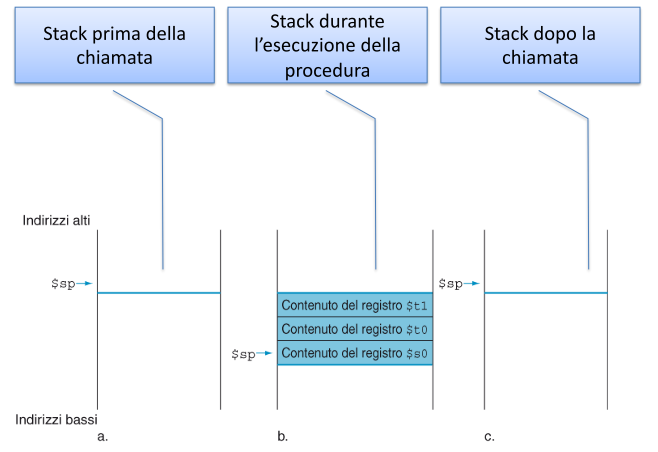
\includegraphics[width=0.9\textwidth,keepaspectratio]{Evoluzione-stack}
\end{figure}

Una volta visto l'esempio vanno fatte deu precisazioni, un compilatore effettivo non avrebbe mai svolto così la procedura poichè:
\begin{itemize}[nolistsep, noitemsep]
	\item I registri temporanei NON devono essere preservati
	\item L'utilizzo di \emph{\$s0} non era necessario
\end{itemize}

Vediamo ora un esempio più complesso dove si affrontano ostacoli come variabili locali e procedure annidate (a detta di tutti temutissime); la soluzione che si applica in questo caso è il salvare nello stack appunto le variabili locali e i valori del registro \emph{\$ra}.

\begin{minted}{c}
   int fact(int n){
	   if (n < 1)
		   return 1;
	   else
		   return n*fact(n-1);
   }
\end{minted}

Vediamo quindi la traduzione del seguente esempio da C ad assembly MIPS:

\begin{minted}{asm}
fact:   #decremento $sp di 8 creando lo spazio per 2 words
		addi $sp, $sp, -8;
	#salvo i registri $ra e $a0 nello stack
	#remind: $ra contiene l'indirizzo di ritorno post-funzione
	#remind: $a0 contiene il dato, in questo caso n
		sw $ra, 4($sp)
		sw $a0, 0($sp)
	#fine del prologo, inizio della procedura effettiva
		slti $t0, $a0, 1
	#$t0 settato a 1 se n < 1
		beq $t0, $zero, L1	#Se n > 1 saltiamo a L1
		addi $v0, $zero, 1	#$v0=1
		addi $sp, $sp, 8	  #Ripulisco lo stack
	#ritorno all’indirizzo dopo la chiamata (n-esima) di fact
		jr $ra
L1:	     addi $a0, $a0, -1 #decremento n
		jal fact	  #chiamiamo fact(n-1)
	#a questo punto ripristino $a0 e $ra e ripulisco lo stack
		lw $a0, 0($sp)	#Ripristino a0
		lw $ra, 4($sp)	#Ripristino ra
		addi $sp, $sp, 8      #ripulisco stack
	#infine moltiplico n*fact(n-1), che è in $v0, e ritorno
		mul $v0, $a0, $v0
		jr $ra
\end{minted}

arrivato a pag. 94



\end{document}
